
\documentclass[conference]{IEEEtran}
% Some Computer Society conferences also require the compsoc mode option,
% but others use the standard conference format.
%
% If IEEEtran.cls has not been installed into the LaTeX system files,
% manually specify the path to it like:
% \documentclass[conference]{../sty/IEEEtran}
\usepackage{graphicx}
\usepackage{cite}
\usepackage{url}
\usepackage{listings}
\usepackage{float,subcaption}
\usepackage{amsmath}
\usepackage{tikz}
\usepackage{multirow}
\usepackage{pstricks,framed}


%\usepackage{subfig}

\usepackage{enumitem}
%\usepackage{IEEEtrantools}
\usepackage{epstopdf}
\graphicspath{{images/}}

\hyphenation{op-tical net-works semi-conduc-tor}


\begin{document}
%
% paper title
% Titles are generally capitalized except for words such as a, an, and, as,
% at, but, by, for, in, nor, of, on, or, the, to and up, which are usually
% not capitalized unless they are the first or last word of the title.
% Linebreaks \\ can be used within to get better formatting as desired.
% Do not put math or special symbols in the title.
\title{Security Vulnerabilities of Unmanned Aerial Vehicles and Countermeasures: An Experimental Study}


% author names and affiliations
% use a multiple column layout for up to three different
% affiliations
%\author{\IEEEauthorblockN{Vishal Dey}
%\IEEEauthorblockA{School of Computer Science and\\Technology\\
%Indian Institute of Engineering\\ Science and Technology\\
%Shibpur, Howrah - 711103\\
%Email: vishal.dd2014@cs.iiests.ac.in}
%\and
% \IEEEauthorblockN{VikramKumar Pudi}
% \IEEEauthorblockA{School of Computer Science and\\Engineering\\
% 	Nanyang Technological\\ University\\
% 	Nanyang Avenue, Singapore 639798 \\
% 	Email: pudi@ntu.edu.sg}
% \and
% \IEEEauthorblockN{Anupam Chattopadhyay}
% \IEEEauthorblockA{School of Computer Science and\\Engineering\\
% 	Nanyang Technological\\ University\\
% 	Nanyang Avenue, Singapore 639798 \\
% 	Email: anupam@ntu.edu.sg}
%}

% conference papers do not typically use \thanks and this command
% is locked out in conference mode. If really needed, such as for
% the acknowledgment of grants, issue a \IEEEoverridecommandlockouts
% after \documentclass

% for over three affiliations, or if they all won't fit within the width
% of the page, use this alternative format:
% 
%\author{\IEEEauthorblockN{Michael Shell\IEEEauthorrefmark{1},
%Homer Simpson\IEEEauthorrefmark{2},
%James Kirk\IEEEauthorrefmark{3}, 
%Montgomery Scott\IEEEauthorrefmark{3} and
%Eldon Tyrell\IEEEauthorrefmark{4}}
%\IEEEauthorblockA{\IEEEauthorrefmark{1}School of Electrical and Computer Engineering\\
%Georgia Institute of Technology,
%Atlanta, Georgia 30332--0250\\ Email: see http://www.michaelshell.org/contact.html}
%\IEEEauthorblockA{\IEEEauthorrefmark{2}Twentieth Century Fox, Springfield, USA\\
%Email: homer@thesimpsons.com}
%\IEEEauthorblockA{\IEEEauthorrefmark{3}Starfleet Academy, San Francisco, California 96678-2391\\
%Telephone: (800) 555--1212, Fax: (888) 555--1212}
%\IEEEauthorblockA{\IEEEauthorrefmark{4}Tyrell Inc., 123 Replicant Street, Los Angeles, California 90210--4321}}




% use for special paper notices
%\IEEEspecialpapernotice{(Invited Paper)}




% make the title area
\maketitle

% As a general rule, do not put math, special symbols or citations
% in the abstract
\begin{abstract}
Drones present a novel airborne platform for new commercial and consumer tasks. Due to their increasing use security analysis has become necessary. In this paper, we present a collection of fatal attacks, minor observations and associated security vulnerabilities for DJI Phantom 4 Pro(P4P) and Parrot Bebop 2 drones.
We also propose some countermeasures to bolster the security of the analyzed drones. In addition to this, we provided a brief overview of the system and embedded architecture of these vehicles. 
 Although DJI has tried to improve security by introducing radio communication and partially encrypted firmware, the P4P still remains vulnerable to GPS spoofing, jamming and other vulnerabilities through DJI-SDK has been exposed in our experimental study. In contrast, Bebop drones are more vulnerable to wireless attacks and we have experimentally validated this for Bebop 2 drone. 
 %In  this paper, we also propose some simple  countermeasure techniques for these  vulnerabilities of the drones.
\end{abstract}

% no keywords




% For peer review papers, you can put extra information on the cover
% page as needed:
% \ifCLASSOPTIONpeerreview
% \begin{center} \bfseries EDICS Category: 3-BBND \end{center}
% \fi
%
% For peerreview papers, this IEEEtran command inserts a page break and
% creates the second title. It will be ignored for other modes.


\section{Introduction}
% no \IEEEPARstart

The demand for unmanned aerial vehicle (also known as drone) technology is rapidly growing \cite{meyerson2015top}. 
%Aerospace research company Teal Group has estimated that sales of military and civilian drones will total over $\$$89 billion in the next 10 years.
Today, drones are increasingly used not only in military applications, but also for civilian tasks \cite{vattapparamban2016drones}, such as delivery services, traffic surveillance, agriculture and farming, aerial surveys, and a variety of tasks that are too dangerous or remote for humans \cite{ruiz2017unmanned,David, corcoran2014drone}. 
It won't be long before drones can also be used in disaster relief, expanding Internet access, and more \cite{David}. 
Recently, The German logistics company, DHL, and Amazon announced the launching of a new drone-based delivery service.
An Australian textbook rental company, Zookal, has already started using drones to deliver
books. 
%Amazon will soon start a new delivery method, Amazon Prime Air, which will use drone-like octocopters %for deliveries. 
Drones have become part of Internet-of-Things (IoT) as well, given the increased use of drones in commercial areas like, agricultural and surveillance, in which vast amounts of visual data are collected from the air and passed to the cloud for analysis using the Internet.

\textcolor{red}{In future, drones ought to replace connected sensors at rest in the IoT, as drones are 1) deployable in different locations, 2) capable of carrying flexible payloads, and 3) re-programmable in mission. Recently Broadcom introduced the WICED Sense Development Kit, an all-in-one IoT prototyping kit for drones. The Erle Robotics company offers Erle-Brain operating systems capable of connecting drones with IoT. 
In a few years, Internet connected drones will be widely used in commercial and civil tasks. 
Because IoT drones are directly accessible over the Internet, require GPS signals and communicates wirelessly, they cause a serious threat to the security of the drone platform.}
For example, a drone-hijacking program called SkyJack was recently engineered to 
autonomously seek out, hack, and wirelessly take over other drones within Wi-Fi distance and turn them into zombie drones under the control of attackers.
Thus, it is critical to address the security of connected (to the Internet) drones. 
 
\subsection{Motivation}
Future smart cities will be swarming with drones for different commercial and personal purposes in the hope that it will improve the lives of humans  \cite{nonami2007prospect}. Drones are harmless when used properly and can be extremely useful, for example, for taking beautiful aerial photographs and cinematography. Although when misappropriated, drones can lead directly to invasions of privacy, concerns with aircraft safety, and even result in personal injury. 

An armed drone used for military purposes can lead to catastrophic results if it gets hacked and lands in the hands of terrorists. Small drones like those used by civilians are even easier to attack; these drones use a wireless transmission protocol for navigation(radio waves or WiFi) and telemetry, and the navigation signals
associated with this are easy to manipulate in order to hack the drone. Attackers may attack drones for a variety of reasons, hacking them to obtain objectionable media, valuable personal information or data.
Companies like Amazon and, Domino’s have planned to deliver items using drones, which, if hacked will not reach the target customer. Given increased popularity and numbers, drones pose an immediate security concern, thus making a security analysis mandatory.

\subsection{Security Issues in Unmanned Aerial Vehicles (UAVs)}\label{Related Works}
We survey the vulnerabilities found in Phantom and Bebop drones, including drone hacks based on unprotected WiFi, access to drone configuration files and, changes to settings in flight, and GPS attacks. 
 
\noindent {\bf WiFi insecurity: } The Parrot drones allow multiple connections through WiFi, which allows an attacker to tamper with the system and hack the drone. 
%We observed different types of wireless attacks on the Bebop2 drone, however these attacks are not applicable to the Phantom 4 Pro as there is no WiFi communication.

\noindent \textbf{SkyJack: }
The SkyJack \cite{skyjack} developed by Samy Kamkar uses a Raspberry Pi and aircrack-ng \cite{aircrack} mounted on a WiFi-based drone, e.g. Phantom 2 Vision or Parrot drones, enabling it to fly, around and get into the network of nearby drones. The SkyJack disconnects the controller by changing the SSID and, immediately reconnects and is then able to transmit commands through the malicious drone to the hijacked drone, enabling it to and take control of other drone in flight using a customized script, hereby forming zombie drones. The DJI Phantom 4 Pro is not vulnerable to this attack whereas the Bebop2 drone is. 

\noindent \textbf{GPS based attacks:}
Drones uses GPS signals for navigation. The GPS signals used by civilians drones are not encrypted. 
Because of this drones are vulnerable to the GPS attacks. The necessary conditions to be met for successful spoofing and different capture and post-capture control techniques demonstrated  in \cite{ROB:ROB21513}.

\noindent \textbf{Maldrone: }
Maldrone\cite{maldrone} sets up a proxy serial port, intercepts flight commands from the controller, and redirects actual serial port communication to fake ports, while forwarding the hijackers commands to the drone. While the Bebop 2 will be affected, this attack is not applicable for Phantom 4 Pro.


\textcolor{red}{In this work, we performed some known experiments like GPS Spoofing, wireless attacks and also exposed new vulnerabilities associated with DJI P4P and Parrot Bebop 2 drones like cracking DJI-SDK, reverse-engineering firmware. Most of the published wireless attacks desribed above are reproduced for Parrot Bebop 2 which proved succesful and the attacks for this drone as presented in Section \ref{Attacks performed} are merely derived from previous attacks.}
The works in \cite{mit9}, several hackers in \cite{defcon23} in DEFCON mainly demonstrated attacks on the DJI Phantom 3 Standard drone. We found that most of the attacks demonstrated are not applicable to the DJI Phantom 4 Pro. Based on our experiments, we found that GPS spoofing is the most prominent attack against the DJI Phantom 4 Pro drone, but it does not affect the Bebop 2 drone. 
% due to .

\textcolor{red}{To the best of our knowledge, there has been no survey review detailing the security issues, embedded architecture and the attacks with thorough explaination for DJI P4P and Parrot Bebop 2 as two drones under study. Our contribution lies in that we provide a detail analysis of the architecture, operation overview, published attacks, new vulnerabilities and also proposed countermeasures. Though we performed our experiments on two drones and specifically mention only two UAVs throughout the paper, most of the attacks will be applicable to drones of similar architecture and communication protocols. e.g. Drones using WiFi for communicating with the ground station controller are vulnerable to attacks similar to Bebop 2. P4P communication is based on RF (radio frequency) technology different from previous builds of Phantom drones, attacks performed in our work are orignial except GPS spoofing.}
    
The rest of paper is organized as follows. Section-\ref{System Overview} provides a detailed analysis of the architecture, internal operations and governing system of the Phantom 4 pro and Bebop 2 drones. 
In Section \ref{Attacks performed} we, describe the experiments conducted on 
 Phantom 4 and Bebop 2 drones to identiy security vulnerabilities: reverse engineering drone firmware, removing authentication from DJI SDK, a GPS spoofing attack on P4P, and wireless attacks. 
A comparison of the  two drones in terms of user-friendliness and security issues is presented in Section \ref{Comparison of two drones}, proposed countermeasures against the security threats are presented in Section \ref{Proposed countermeasures}. In section~\ref{sec:conclusion}, we conclude and discuss future work. 


\section{DJI Phanthom 4 and Parrot Bebop 2 Drones Architecture and Operation Overview}\label{System Overview}
In this section, we provide a detailed description of the internal architectures, internal operations, and operating system of DJI Phantom 4 Pro and  Parrot Bebop 2 drones. 


\subsection{DJI Phantom 4 Pro}
 A brief overview of the DJI Phantom 4 Pro drone system and its components follows. 
\begin{figure}[h!]
	\centering
	\begin{subfigure}{.23\textwidth}
		\centering
		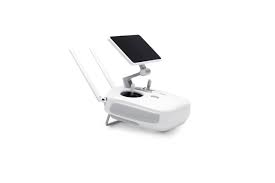
\includegraphics[width=0.9\linewidth]{rc}
		\caption{Controller with phone}
	\end{subfigure}
	\begin{subfigure}{.23\textwidth}
		\centering
		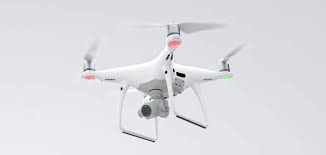
\includegraphics[height=0.11\textheight, width=0.9\linewidth]{drone}
		\caption{Phantom 4 Pro}
	\end{subfigure}
		\caption{DJI Phantom 4 Pro with controller}
		\label{fig:Phantom4}
\end{figure}

%include picture
The DJI Phantom 4 Pro drone consists of a remote controller, mobile device and drone components as shown in Fig.~\ref{fig:Phantom4}. 
The remote controller is a multifunction wireless communication  device with Lightbridge technology that integrates a dual frequency video downlink system and the aircraft remote control system. 
The mobile device uses the DJI GO 4 app which acts as a user-friendly interface to control the drone and displays the live video feeds. 
It has many advanced features such as RTH(return-to-home), Waypoint mission and other intelligent flight modes including TapFly (to fly in the designated position without using the remote controller), ActivTrack
(to mark/track a moving object on the mobile screen, e.g., tracking a car in a race), and Draw (for Waypoint missions).
The drone itself is a major component of the system, and it receives commands and sends data to the mobile device using radio signals with frequencies of 2.400 GHz - 2.483 GHz and 5.725 GHz - 5.825 GHz ISM bands.


The DJI Phantom 4 Pro operates using the Rockchip ARM-processor and Unix-based operating system, BusyBox. 
It comes with a powerful remote controller that has Lightbridge technology. Lightbridge is a one way stream of data without two way handshaking, minimizing video latency while maximizing flight distance.
As a result, latencies with Lightbridge are more consistent at a distance versus standard WiFi. Lightbride is much faster at re-establishing a connection when it reaches it’s distance limit. The GL300 main board is the most important hardware component, supporting the processor, Ambarella, CPU, FPGA Altera Cyclone V, microSD slots, radio transceiver modules, etc. 

%The OFDM Receiver module is responsible for pairing with RC and communicating with it. 
%It comes from Orthogonal Frequency Division Multiplexing - which is a way of transferring broadband data. 
The OFDM receiver implements the Lightbridge technology, and is also a middleman between the gimbal and flight controller. The control and video is transmitted over 2.4 GHz using digital transmission for the video along with the standard 'packet' style control link with the usual parity and identity confirmation checks over the frequency hopping spread spectrum.
Ambarella makes a video stream to the davinchi module via HDMI (or USB) and at the same time writes a video stream to microSD (using video compression H.264 or H.265). Then DaVinchi sends video to the Encryption module, after that encrypted stream goes to RF transceiver (AD9364).
The u-blox NEO GPS chip, which has the ability of J/N monitoring, is used.
%hardware picture

\subsection{Parrot Bebop 2}
The Parrot Bebop 2, an easy-to-fly user-friendly drone, is shown in Fig.~\ref{fig:beebop2}. The Bebop 2 drone setup requires a drone and mobile device. 
The mobile device uses ``FreeFlight Pro," an official app, for control and communication of the drone.
The mobile device binds to the network and, establishes a connection with the drone via Wi-Fi.  It sends drone commands and 
receives drone data and other sensor readings and sends video packets over UDP. The drone acts as an 802.11 Wi-Fi hotspot for 2.400 GHz - 2.483 GHz and establishes a Bebop network once powered on.  Both the controller and the drone maintain their open access points(APs) active.

%include picture
\begin{figure}[h!]
	\centering
	\includegraphics[width=0.4\columnwidth]{beebop2.jpg}
	\caption{Parrot Bebop 2 drone}
	\label{fig:beebop2}
\end{figure}


Bebop 2 uses a P7 dual core CPU, a quad-core GPU, and 8 GB of memory, and the operating system is a striped down version of Unix: BusyBox. The Bebop2 OS, AR Drone 3 maintains the typical UNIX filesystem hierarchy, as well as its open architecture.
The Bebop memory is accessed through its WiFi connection and the use of communication protocols such as Telnet ​and FTP. 
The onboard flight controller controls the drone by combining input from several sensors, including a {\it GPS chip} (Furuno GN-87F GPS chip or u-blox Neo 8M), a {\it vertical camera} (MT9V117 camera) used for adjusting of the Bebop drone's orientation and XY position, and other sensors (e.g. barometer, accelerometer, and magnetometer etc.) for assistance.

%\paragraph{GPS chip} After removing the Bebop plastic nose, the Furuno GN-87F GPS chip(or Ublox Neo 8M) is located on top of the camera mount block. 
%\paragraph{Others} The ​MS5607​ barometer mounted 
%onboard the Bebop has a known problem with light: when hit by strong light, the barometer undergoes a sudden shift. There are other sensors like accelerometers and magnetometers for assistance.
%\paragraph{Vertical Camera} The vertical ​MT9V117​ camera shoots a frame every 25 ms. Using these frames the software adjusts the Bebop orientation and X­Y position. 



\section{Attacks performed}\label{Attacks performed}

\subsection{DJI Phantom 4 Pro}
\subsubsection{Cracking DJI SDK}
DJI provides mobile and on-board SDK which are available for download from \cite{djisdk}.
This attack is based on the removal of authentication between the DJI app and the DJI server. DJI offers an SDK to build customized Android and iOS apps. This enables to modification of the SDK by decompiling and patching portions of code. The first use of DJI Go or any customized app using DJI-SDK, requires one time registration and activation. 

%\begin{figure}[h!]
%	\centering
%	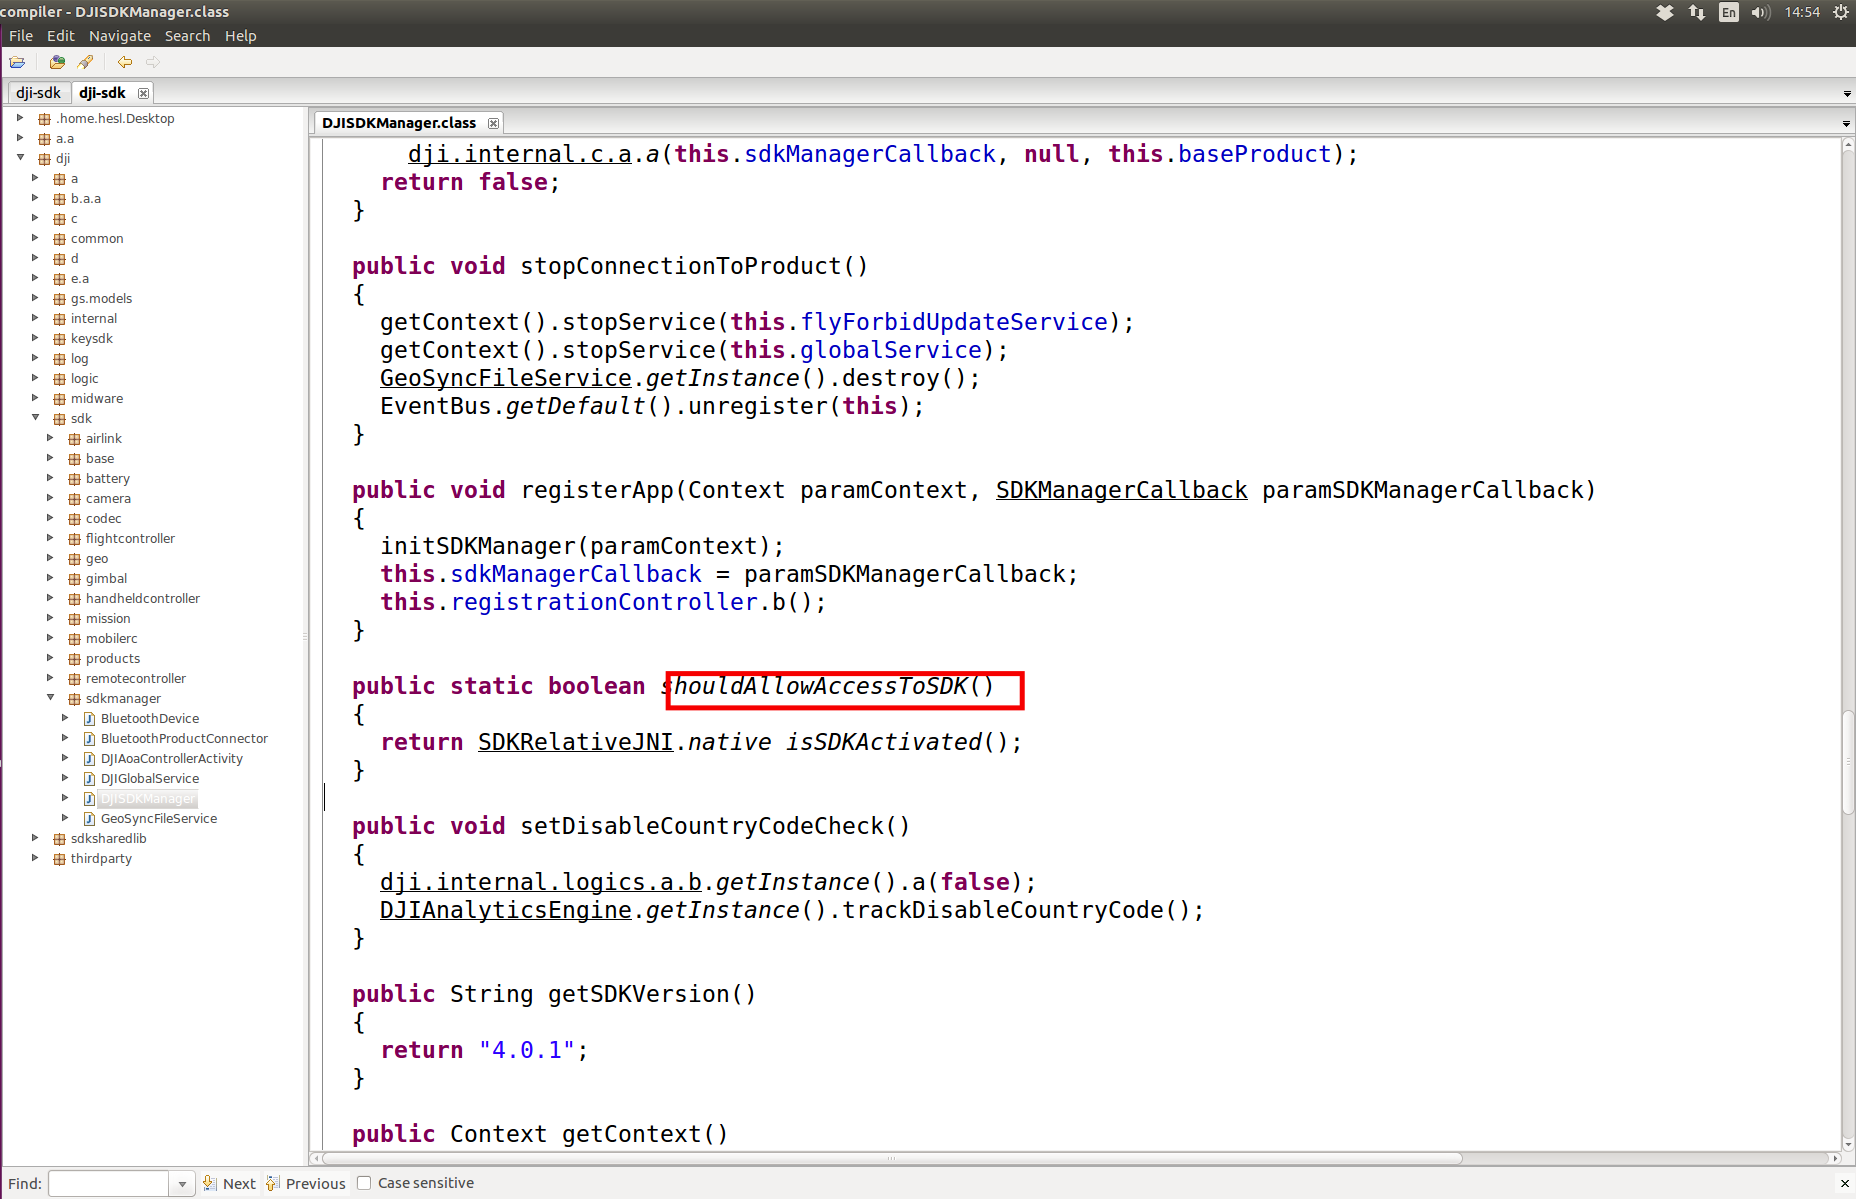
\includegraphics[width=0.9\columnwidth]{jd}
%	\caption{Portion of decompiled SDKManager Class}
%\end{figure} 

We decompiled the library jar file dji-sdk using \cite{jdgui} and edited the code using \cite{jbe}. 
We found that the following functions largely handle this authentication: registerApp, isSDKActivated,  shouldAllowAccessSDK and hasSDKRegistered. startConnectionToProduct(). These functions calls shouldAllowAccessSDK(), checks whether the user will be given access to SDK. The hasSDKRegistered() function registered with a valid AppID(key) against a registered user, which is obtained after registration of an app. This key is pasted as an AppID in the main Manifest.xml file of the customized app to activate DJI-SDK.
%\begin{figure}[h!]
%	\centering
%	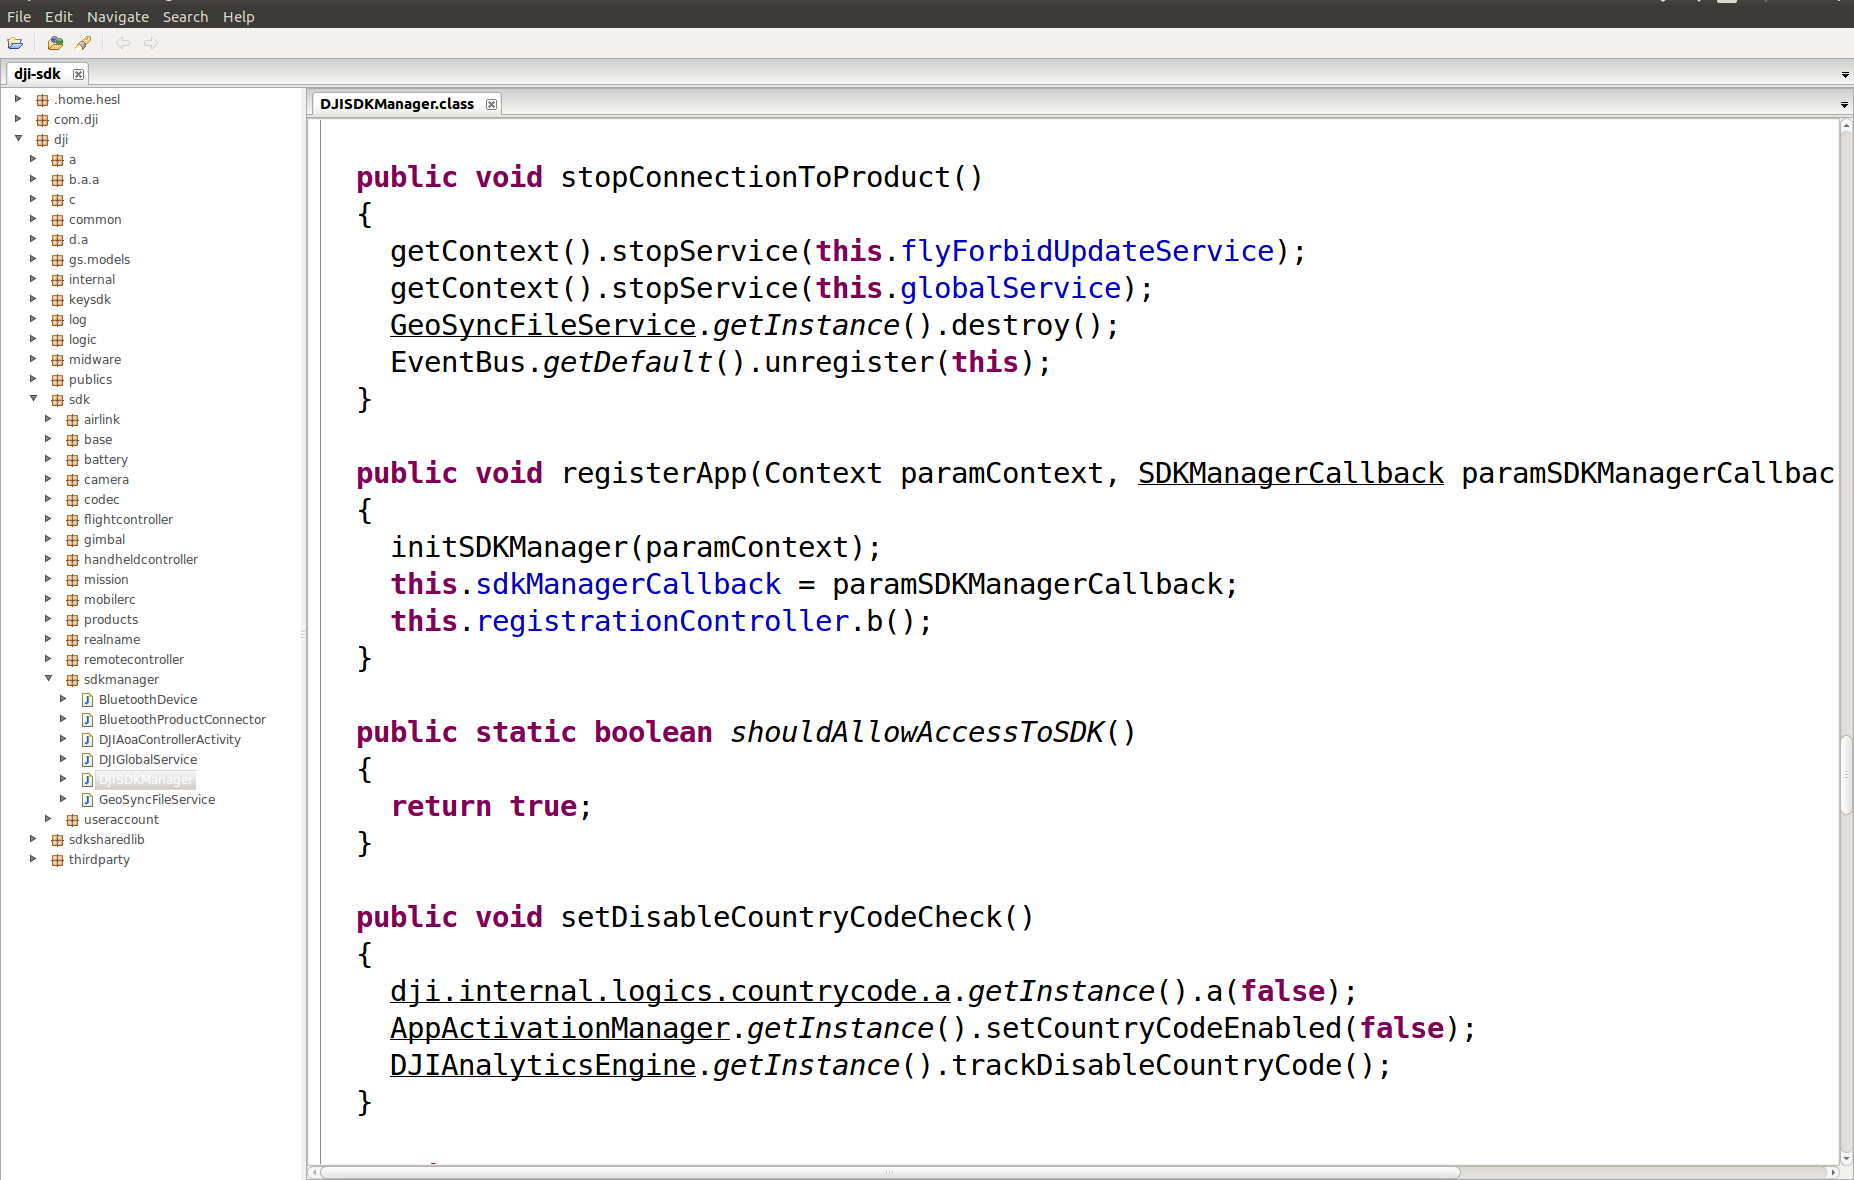
\includegraphics[width=0.9\columnwidth]{jd1}
%	\caption{Patched code for shouldAllowAccessSDK}
%\end{figure}

We patched two functions(shouldAllowAccessSDK() and hasSDKRegistered()) to return true always without any further permission checking, thus effectively removing authentication. Therefore even a wrong key or null string used as the AppID would not result in an error that would prevent the app from opening.
This authentication is crucial in preventing malicious users from taking control of a drone away from an authentic user.
We built custom apps for controlling the camera and, taking photos and, videos, and a playback manager, using the cracked SDK. The custom apps were successfully authenticated and, worked perfectly fine.
%screenshots

\begin{figure*}[!hbt]
	\centering
	
	
	\begin{subfigure}{.45\textwidth}
		\centering
		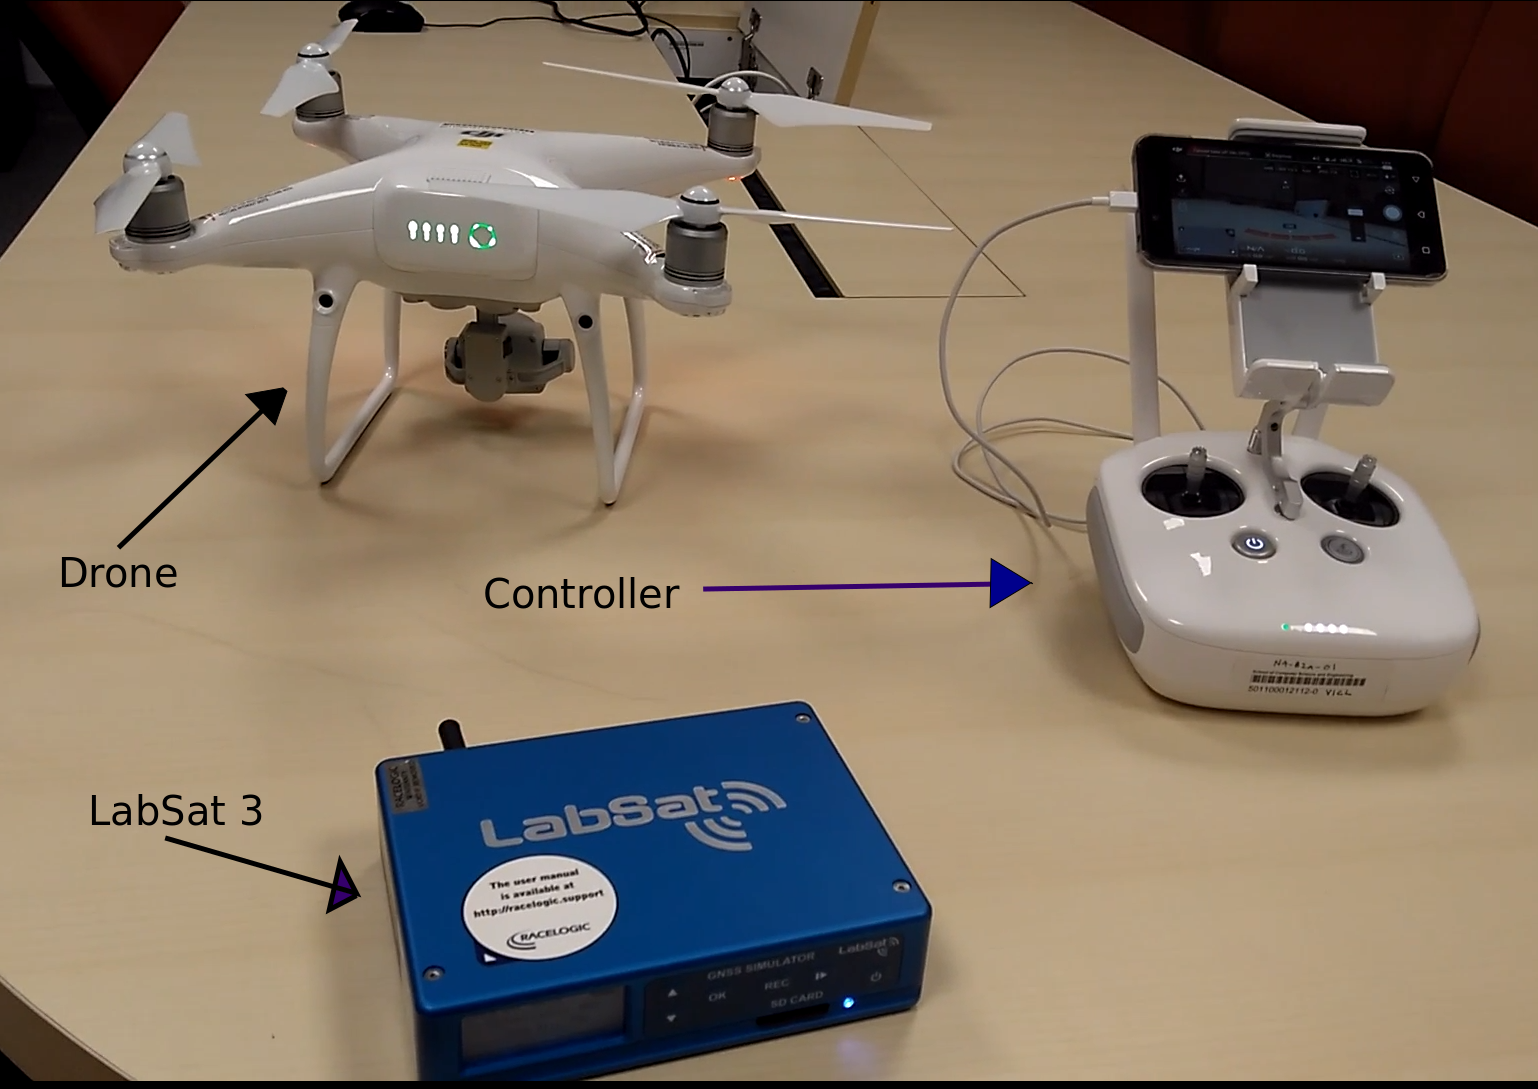
\includegraphics[width=0.7\columnwidth]{images/setup} 
		\label{fig:setup}
		\caption{GPS Spoofing Setup for DJI Phantom Drone}
	\end{subfigure} \hfil
	\begin{subfigure}{.45\textwidth}
		\centering
		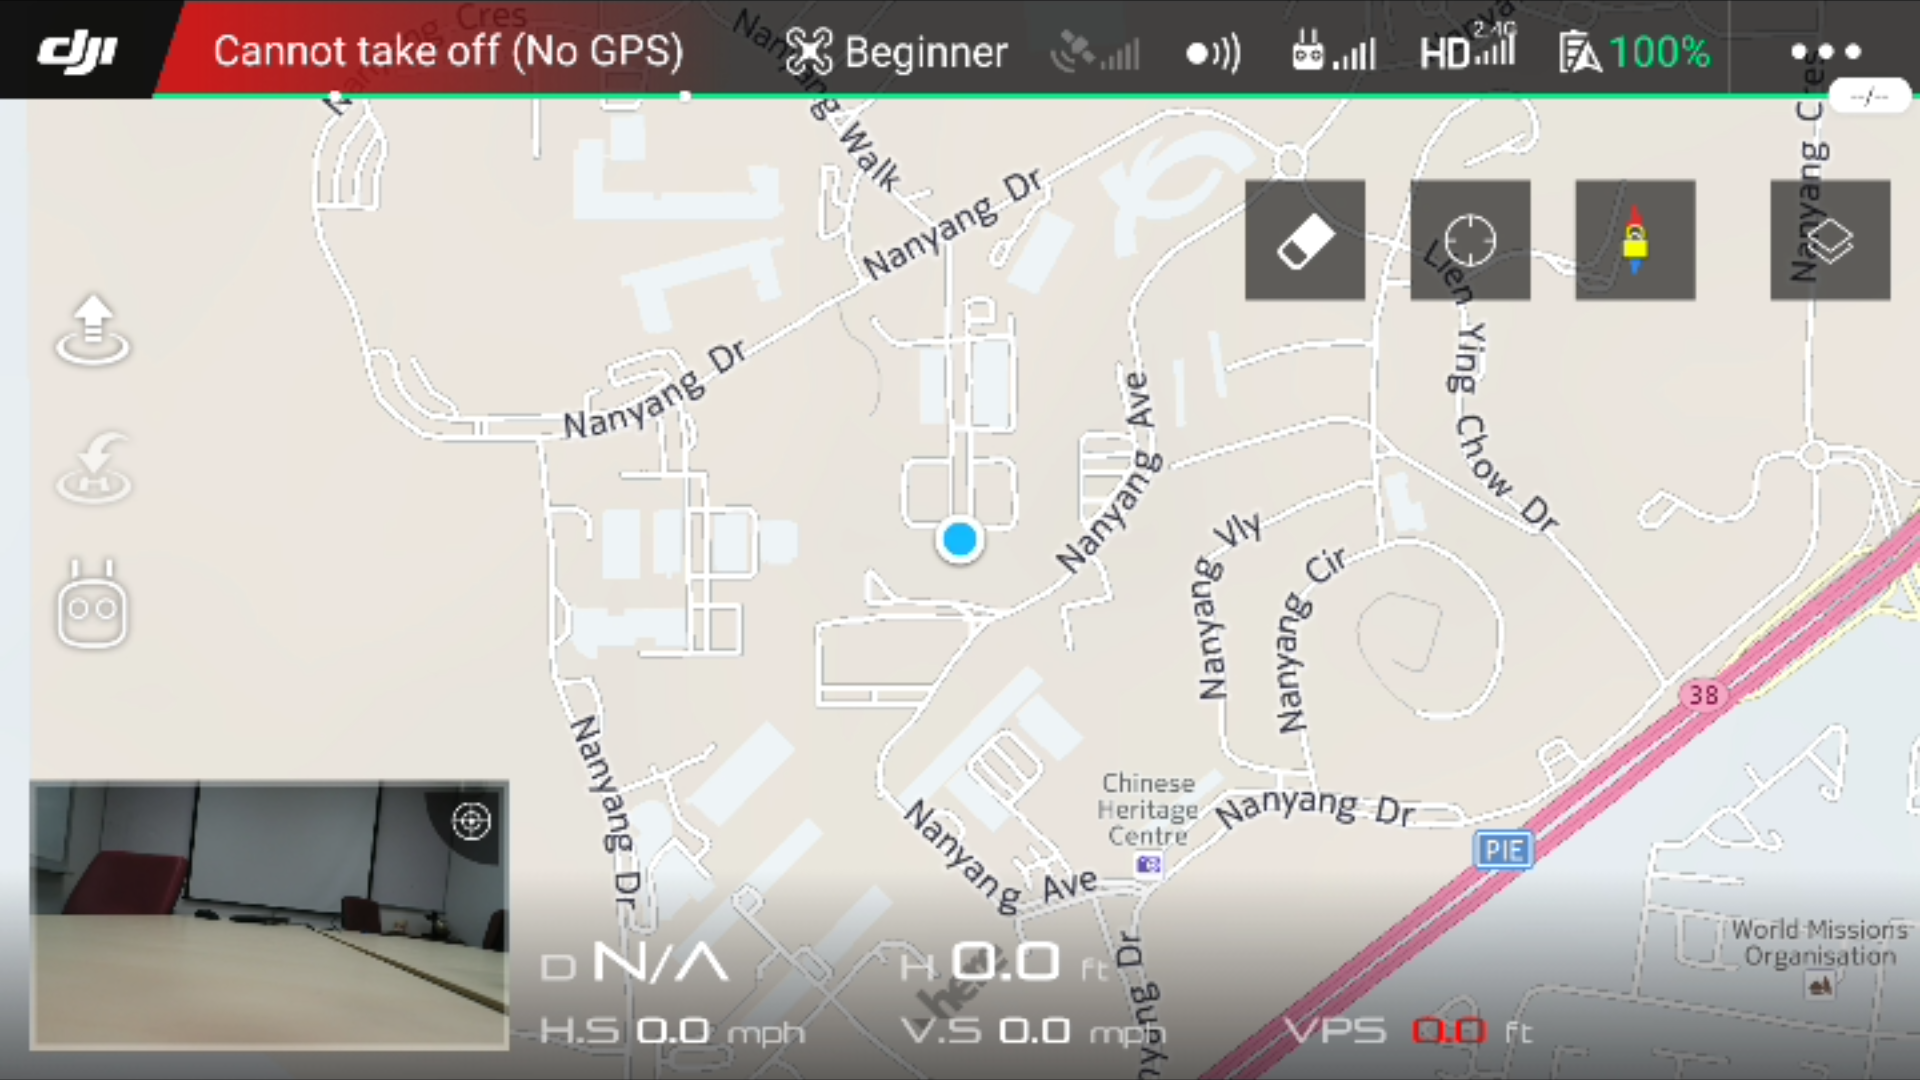
\includegraphics[width=0.8\columnwidth]{ntu}
		\caption{Original Location of Drone (NTU, Singapore)}
		\label{fig:ntu}
	\end{subfigure}\\	
	\begin{subfigure}{.45\textwidth}
		\centering
		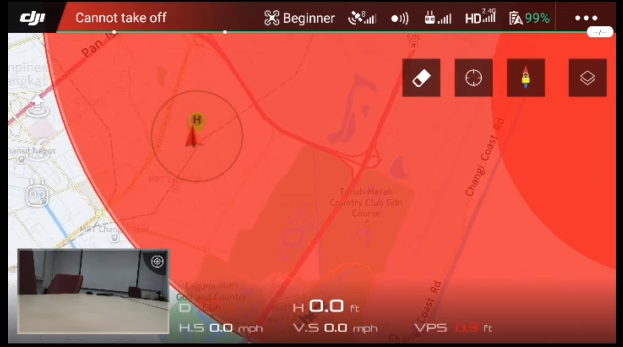
\includegraphics[width=0.8\columnwidth]{nfz}
		\caption{No Fly Zone near SUTD, Changi Airport}
		\label{fig:nfz}
	\end{subfigure} \hfil
	\begin{subfigure}{.45\textwidth}
		\centering
		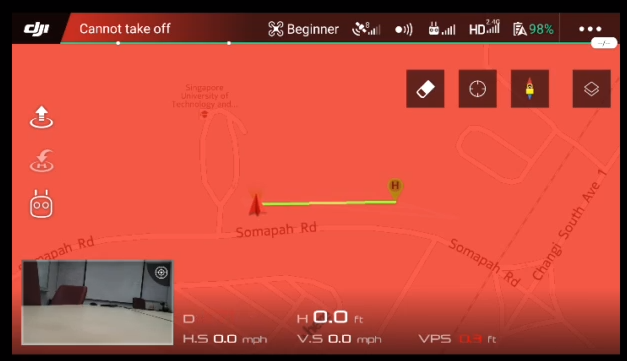
\includegraphics[width=0.8\columnwidth]{moving}
		\caption{Drone Spoofed Location Movement}
		\label{fig:drone mov}
	\end{subfigure}
	
	
	\caption{DJI Phantom Drone GPS Spoofing Experimental Setup and Drone GPS Spoofed Locations }	
	\label{fig:Hist_EM}		
\end{figure*}


\subsubsection{Reverse Engineering Firmware}
The binary of the DJI Phantom 4 Pro firmware is encrypted and digitally signed. 
We ran a customized parser to unpack the firmware. 
We unpacked firmware using RKflash \cite{rkflash} : a flashing tool for Rockchip based systems, and obtained standard images.
The image \emph{embedded-update.img} was further extracted into standard image modules: \emph{boot.img}, \emph{recovery.img}, \emph{system.img}.
We further unpacked into standard Android partitions using different Android image flash tools.
Although we were able to decrypt the binary, it was not possible to reflash DJI Phantom 4 Pro with the new binary.
This is likely because the binary is not completely decrypted. 
%\begin{figure}[h!]
%	\centering
%	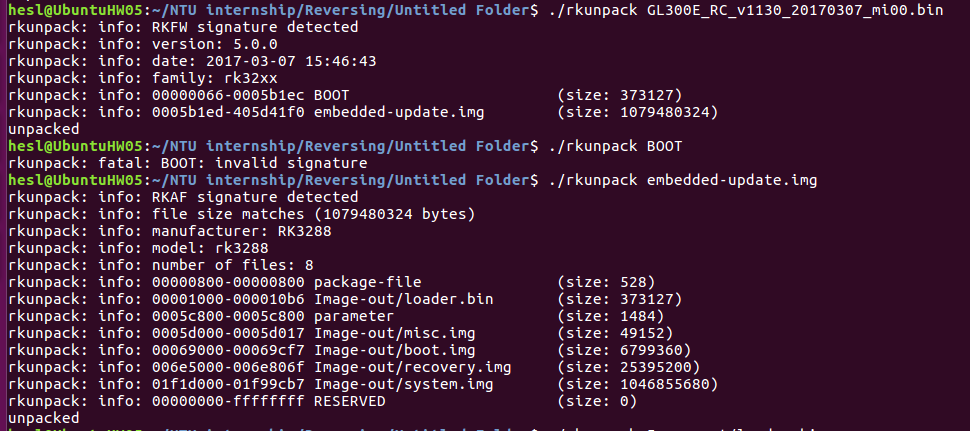
\includegraphics[width=0.9\columnwidth]{rkunpack}
%	\caption{Standard Android partitions obtained}
%	\label{fig:reversing}
%\end{figure}
%screenshots

\subsubsection{GPS Spoofing}
DJI Phantom drones are GPS based drones. 
%receiving incoming signals from GPS satellites, signals notifying the drone’s presence, and a two-way link between the ground station controller and the drone.
GPS enables a drone’s navigation, and due to the lack of encryption of the civilian GPS signals, they can be easily spoofed. The basic idea in GPS spoofing is the transmission of fake GPS coordinates to the flight controller of the drone.
This will enable an attacker to hijack the drone and place it in the complete control of the attacker.
To spoof a GPS receiver, a transmitter is used to transmit false GPS signals, forcing the drone GPS to synchronize with the attacker’s signals, including spoofed information regarding the ephemeris and almanac data. 
If the GPS receiver switches from legitimate GPS signals to false GPS signals, causing the drone to veer off its path and sending the drone in a direction specified by the attacker. 
%A successful attack is conducted when attacker is very close to the drone, or by using a directional antenna of proper frequency aiming the drone.


Though DJI improved the navigation by utilizing inertial measurement unit(IMU) in its drones, instead of relying only on GPS, we still managed to spoof the GPS receiver using the LabSat3 GPS simulator\cite{labsat}. 
DJI Phantom 4 Pro comes with the u-blox NEO 8M GPS receiver which has the ability to detect jamming with the help of J/N monitoring. 
J/N monitoring triggers an alarm if the received power is more than the triggering threshold, preventing a jam-and-then-spoof kind of attack. 
We performed the spoofing attack inside a screened environment (shielded room) in the presence of weak real GPS signals.
It was difficult to conduct the experiment outdoors due to the presence of strong legitimate GPS signals.
%%Explain our setup
\paragraph*{Experimental Procedure}
%Here we perform record and replay attack only. 
First, real GPS signals are recorded using the active antenna RLACS198 provided with the LabSat kit.
We can also generate fake GPS signals using SatGen software provided with LabSat. 
The location of the drone was successfully spoofed by LabSat. 
The drone was placed inside the HESL lab at Nanyang Technological University (NTU).
Although the DJI Phantom 4 Pro has a u-blox GPS module with J/N monitoring, it failed to detect spoofing in our case, because the transmitted power was very low. 
The location, altitude, and speed are provided by the DJI Go 4 app.
In our experiments several kinds of hacks were performed: force landing a drone spoofing the location so as to misdirect the drone to NFZ, flying a drone in a NFZ, and a height hack.
In figure \ref{fig:ntu}, the drone is seen to be located at NTU, the spoofed location shows the drone to be in Changi South Avenue near SUTD in figure \ref{fig:nfz}, which is a no-fly-zone.  
Once spoofed, the drone could perform an emergency landing or 
%If it had been flying with real GPS, and we transmit fake GPS, and these are more stronger in quality than real ones and the spoofed location is a
%NFZ, the drone would perform an emergency landing.
%Similarly the reverse experiment could be performed where the drone was located in a NFZ preventing the drone to take-off and if location is successfully spoofed to a non-restricted place, drone would take off.
the movement of the drone could be faked by replaying a pre-recorded GPS data using LabSat as in figure \ref{fig:drone mov}.

\subsection{Parrot Bebop 2} \label{sec:Bebop_attacks}
Most of the attacks on the Parrot Bebop 2 drone conducted in our experiments are targeted at the open WiFi. 
The Parrot manufacturers introduced the feature of adding the WPA/WPA2 password to the Bebop's WiFi which obviously decreases range and speed. Nonetheless, it remains vulnerable to WiFi attacks. 
Weak password can easily be cracked by tools like \cite{aircrack}.

\noindent \paragraph*{Network Mapping}
The Nmap utility shows the drone’s ports and the different services running on these ports utilizing it. 
Based on the Nmap scan of the drone's IP, we identified three open ports running the following services FTP, Telnet, and Tor-SOCKS.
%\begin{figure}[h!]
%	\centering
%	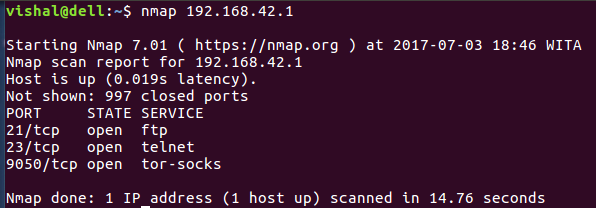
\includegraphics[width=0.9\columnwidth]{nmap_scan}
%	\caption{Nmap scan of IP: 192.168.42.1}
%	\label{fig:nmap}
%\end{figure}
%include picture

\subsubsection{Open WiFi}
The Bebop 2 drone uses an IEEE Wi-Fi radio (802.11ac), and the IP address of the drone is 192.168.42.1. 
An unencrypted open Wi-Fi allows any one to connect the Bebop 2 drone and hijack the drone. Since Bebop2 allows for multiple clients to connect to the network, the problem is more critical i.e. more than one user can control the drone and there is no way of validating the original owner. 

\subsubsection{Deauthenticating Owner}
We performed the deauthentication attack on the drone using method presented in \cite{aircrack}.
This attack consists of capturing packets of the Bebop network without even connecting to drone, thereby disconnecting the authenticated owner.
Initially the wireless network is scanned in monitor mode using airmon-ng. After the Bebop network is found, it snoops into the network using airodump-ng capturing all the packets from that network only. 
%\begin{figure}[h!]
%	\centering
%	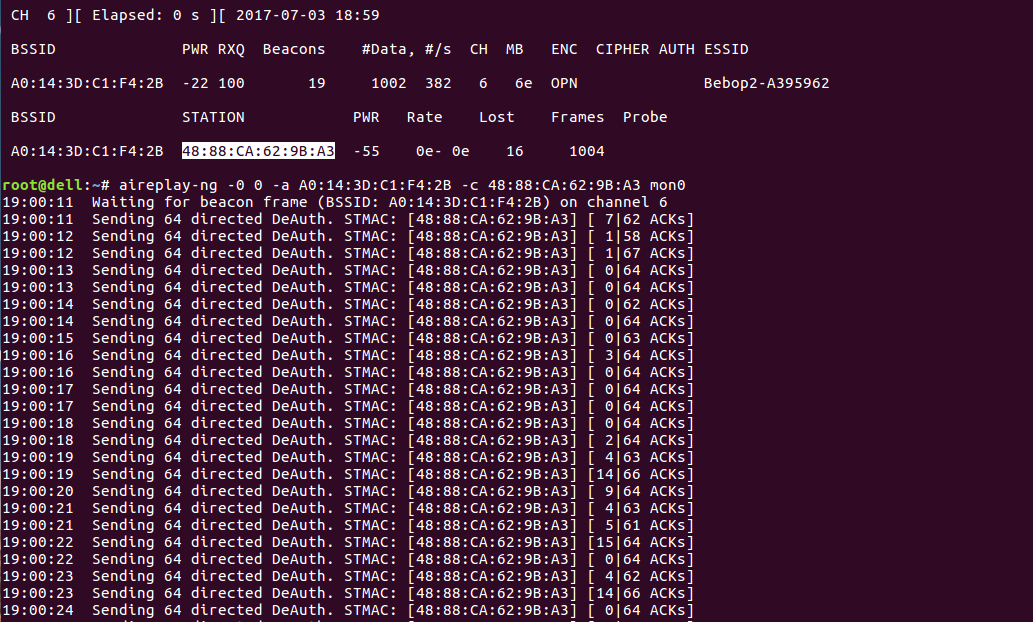
\includegraphics[width=0.9\columnwidth]{deauth}
%	\caption{Deauthenticating the owner}
%	\label{fig: deauth}
%\end{figure}
When the list of clients is available, a deauthentication attack is performed by executing aireplay-ng, which sends de-authentication packets continuously to the clients, disconnecting them until the program executes.
In the meantime, the hacker is able to get connected and as the only client connected, 
can hijack the drone.

In our experiments, the deauthentication packets are sent continuously from the attacker's laptop to the connected client whose MAC address is 48:88:CA:62:9B:A3 where the drone's BSSID is A0:14:3D:C1:F4:2B.
The entire network can be jammed by sending deauthentication packets continuously, preventing anyone from connecting to the network. 
Aireplay-ng sends 128 deauthenticate packets: 64 packets to drone BSSID and 64 packets to the client. 
%In each last column of figure \ref{fig: deauth}, first number denotes the number of ACKs received from the client and second denotes that received from the drone.

\begin{figure}[!hbt]
	\centering
	\begin{subfigure}{.2\textwidth}
		\centering
		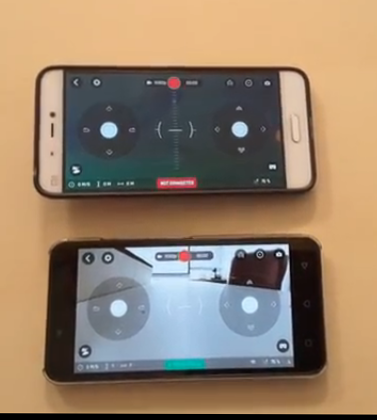
\includegraphics[width=0.85\columnwidth]{disconnec1}
		\caption{Owner Connected}
	\end{subfigure}$\xrightarrow[\text{Deauth.}]{\text{After}}$
	\begin{subfigure}{.2\textwidth}
		\centering
		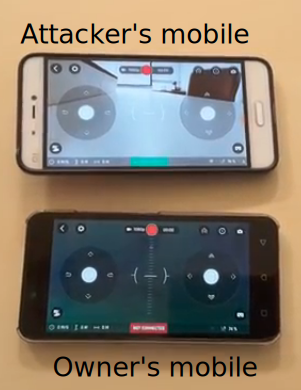
\includegraphics[width=0.85\columnwidth]{disconn2}
		\caption{Owner disconnected}
	\end{subfigure}
	\caption{Deauthenticating owner's mobile}
	\label{fig:disconnect}
\end{figure}

In Figure \ref{fig:disconnect}, the mobile phone belonging to the owner (bottom) remains disconnected as long as aireplay-ng continues to send directed deauthenticate packets.
The attacker takes advantage of this to connect his/her own mobile phone(above) and can now use it to hijack the drone.  

\subsubsection{Open Telnet}
Once connected to the Bebop 2's Wi-Fi, the user can Telnet to it. The drone's IP address is 192.168.42.1. Since multiple users can connect to the drone's Wi-Fi, just attempting to connect to the network, generates multiple requests in a short span of time, which may cause a \textbf{DoS} attack, resulting in an interruption of the original commands.
Even by telnetting to it, the user obtains root access to the entire file system. 
By telnetting into the drone, we were able to kill the main process (\textit{dragon-prog} the main Bebop process governing the whole system of flight control), which would stop motor arms immediately, causing the drone to fall to the ground.
We also found a list of other interesting processes running by \emph{ps} command of UNIX. We also found important shell scripts \emph{/usr/bin/ardrone3\_shutdown.sh} and \emph{/usr/bin/DragonStarter.sh}
We observed that executing \emph{ardrone3\_shutdown.sh} also stopped the main process shutting down the 
drone immediately. 

\subsubsection{Root Access to File System}
Since the release of the Parrot AR.Drone 3.0, most of the files are read-only, except the /data directory which is the FTP media directory.
Though the files are read-only by default, the attacker can override this by remounting the entire file system with
\begin{lstlisting}[language =  bash]
# mount -o remount, rw /
\end{lstlisting}

%\begin{figure}[h!]
%	\centering
%	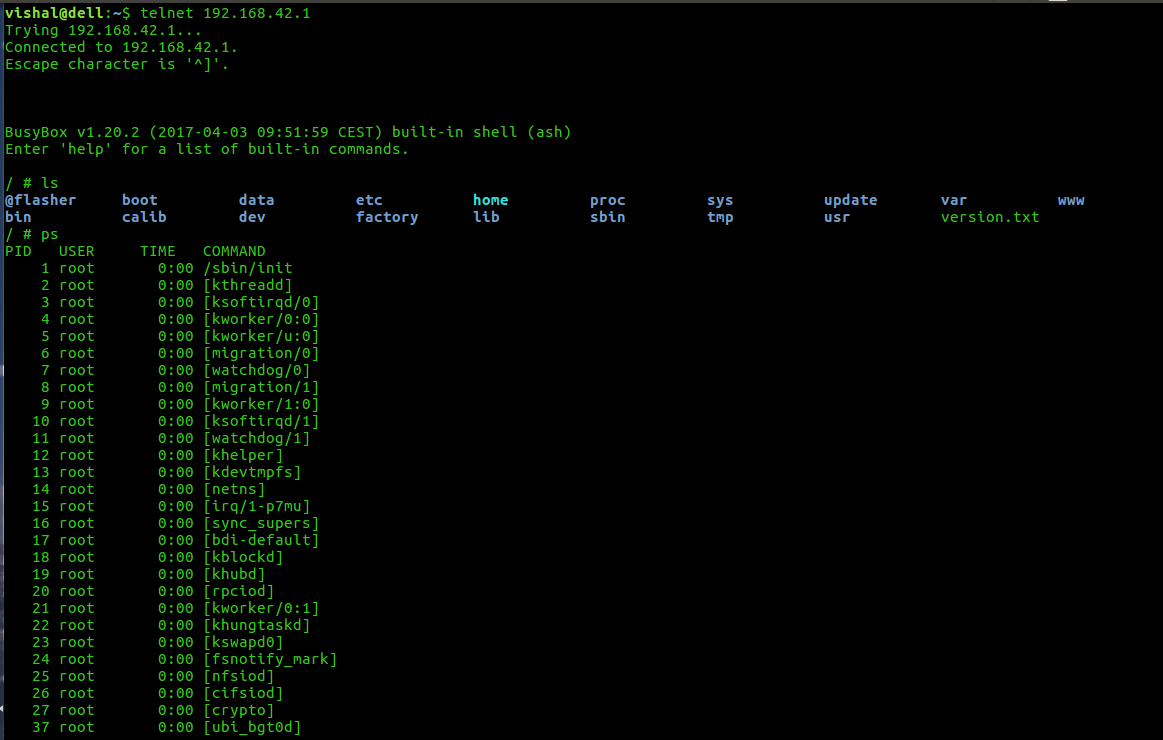
\includegraphics[width=0.9\columnwidth]{root_fs}
%	\caption{Root access to file system}
%	\label{fig:root_fs}
%\end{figure}
%list of interesting files

\subsubsection{Open FTP Port}
Without any authentication for FTP, attackers may connect to the WiFi and login to the FTP to steal personal information including media, flight data, etc.
Based on the factory settings, FTP access does not allow access to the entire files system, and only allows access to the FTP directory \emph{/data/ftp/internal\_000}, which is where images and videos are recorded,  along with other useful files (e.g. pud files).
The limited FTP access can be taken over by the attacker by editing the file \emph{​/etc/inetd.conf}. ​
After the following lines, 
\begin{quote}
	21 stream tcp nowait root ftpd ­wSS /data/ftp
	\linebreak 
	51 stream tcp nowait root ftpd ­wSS /update
	\linebreak 
	61 stream tcp nowait root ftpd ­wSS	
\end{quote}
we need to add the following line to obtain access to the entire file system:

\emph{71 stream tcp nowait root ftpd ftpd ­SS /} 

\subsubsection{Snooping into the WiFi and Packet Capture}
We used Wireshark to capture packets during the connection establishment and throughout the entire flight. The flight commands and video are passed as UDP packets, while the initial connection setup is done by TCP. 

%include wireshark screenshots

\subsubsection{Additional Vulnerabilities}
\paragraph{Reversing firmware}
The Bebop 2 firmware is completely reversible and can be easily modified and the new binary can be reflashed. Reversing firmware gives insight into the drone workflow and file system, which makes it easier for the attacker to exploit vulnerabilities and target specific locations.
\paragraph{Modifying Files}
The entire file system can be accessed using Telnet after being connected to the Bebop's Wi-Fi.
The incorrect modification of configuration files/scripts such as dragon.conf to crash the software and hamper normal drone operation. 
Modifying the /etc/passwd file may brick the drone as changing some passwords may limit the owner's ability to telnet into it, or connect to the drone.

\section{Comparison of two drones}\label{Comparison of two drones}
From our experiments and keen observations made after analyzing the security aspects of both the Phantom 4 Pro and Bebop 2 drones, we found that Phantom 4 Pro drone is more secure than Bebop 2 drone.
Phantom 4 Pro is only vulnerable to GPS spoofing and interception/jamming of radio signals using SDR.
Bebop 2 is prone to various wireless attacks and can be easily hijacked.
While SDR equipment and/or GPS spoofers can be difficult to acquire, due to limited availability and cost, several wireless tools and network scanner, analyzers are readily available online at no cost. 
In addition, it appears that DJI has tried to improve the security of its drones by introducing communication and video feed transmission via radio signals and DJI claims to have an on-board FPGA video encryption algorithm which can be easily verified by scanning transmitted radio signals using SDR or tapping the output of FPGA before it goes to the transceiver. 
DJI also partially encrypts the firmware, and the binary is digitally signed, although it can be decrypted to some extent. 

\section{Proposed Countermeasures against the Drone Security Vulnerabilities}\label{Proposed countermeasures}
In this section,  we propose some methods/actions that can be implemented to increase the security of drones. 
Drones will remain vulnerable to GPS spoofing unless receivers gain the capability of detecting spoofing (e.g. SAASM used by military) thus, there is a need for developing anti-spoofing and anti-jamming receivers.
While there has been a lot of promising work and methods proposed  for the detection and avoidance of civilian GPS anti-spoofing and anti-jamming in the literature similar to that in \cite{wesson2012straight}.
Those methods can be broadly classified into cryptographic (spread spectrum, dual receiver correlation), and non-cryptographic (antenna array). These methods are either difficult to implement or require costly hardware. Therefore we propose some simpler software-based techniques for spoof detection.

\paragraph*{Checking latency}
The motion speed can be validated for a change in location in just a brief instant, (e.g. an individual cannot travel and change his/her location from New York to Beijing in a few seconds).
The changes of coordinates can be recorded and validated given the time it takes to change the coordinates.

\begin{figure}[h!]
	\centering
	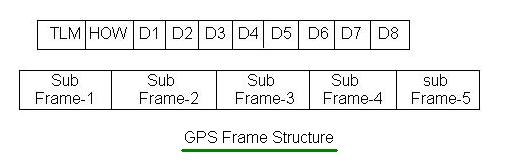
\includegraphics[width=0.7\columnwidth]{gps.pdf}
	\label{fig:gps_frame}
	\caption{GPS frame structure}
\end{figure}

\paragraph*{Checking GPS Subframe Data}
The GPS frame starts with a telemetry word used as preamble, which provides details of the satellite.
Handover word(HOW) provides the GPS system time. HOW is followed by eight data words with parity bits.
Subframe-1 carries information to correct the satellite clock. Subframe-2 and subframe-3 provide ephemeris data for the satellites. 
Subframe-4 and subframe-5 send the almanac data. 
GPS subframe data can be validated easily by checking each of the subframes.
Fake GPS data has been found to have incorrect subframe data, 
thus it is possible to detect spoofing. 
As a countermeasure that can be used to easily detect GPS spoofing, we propose using an onboard Raspberry Pi on the drone to validate time-motion or GPS subframe data. \textcolor{red}{This adds an extra overhead for checking GPS data before passing to the flight controller which affects the latency of the system.}

In addition to GPS anti-spoofing and anti-jamming, we recommend some modifications which can improve the security of drone. 
\begin{itemize}
	\item Using encryption/packer to protect library files
	\item Using an obfuscator to prevent decompiling and, reverse engineering of the firmware
	\item Improve SDK authentication, (although this is, now being done between the app and server, the drone must also be included in the one-time authentication)
	\item Encrypt the entire firmware binary, and store, the encryption key in the hardware
\end{itemize}
\textcolor{red}{These above mentioned strategies are proposed to be implemented by the manufacturer and we left these as recommendations.}

In contrast, many of the attacks described in section~\ref{sec:Bebop_attacks} for Bebop 2 are possible only due to open WiFi and open ports. In addition, FTP need not be activated inflight in order to prevent theft of flight data and media. 
The backing up of Bebop 2 drone data offline provides security for personal data.
For the Bebop 2, and other Wi-Fi based UAVs, we propose the following countermeasures:

\paragraph{Adding WPA security}
The parrot Bebop 2 developers added WPA/WPA2 security to the WiFi using Freeflight Pro app.
Even though it is possible to crack the Wi-Fi password using tools like Aircrack-ng. Still adding WPA to Wi-Fi improves the security of the parrot Bebop 2 drone.
This security improvement may cause decrease in range and transmission speed.

\paragraph{Adding Telnet Password}
Bebop 2 should not allow root access to the file system once connected and telnetted. This can be managed by adding a Telnet password modifying \emph{/etc/passwd} file. 
\paragraph{MAC-Filtering and Hidden SSID}
These can be achieved by installing bcmwl program in the drone. bcmwl controls all of the wireless wi-fi connectivity of the drone. Any changes made can be temporary or permanent. In order to reversibly hide the Wi-Fi SSID, the user can open a Telnet session and enter the following command:
\begin{lstlisting}
  # bcmwl closed 1
\end{lstlisting} 
This makes it more difficult for others to connect to the drone, since the Wi-Fi network will not appear in the list of available networks.
To activate MAC address filtering, enter the following command 
\begin{lstlisting}
  # bcmwl mac MA:CA:DD:RE:SS:01 MA:CA:DD:
  RE:SS:02 ...
\end{lstlisting} 
where all the possible MAC addresses are provided by the owner followed by:
\begin{lstlisting}
  # bcmwl macmode 2
\end{lstlisting} 

which sets MAC filtering to only accept connections from the previous list of devices. To permanently introduce these changes, the \emph{/sbin/broadcom\_setup.sh} file must be modified.\\
\textcolor{red}{Adding these security countermeasures in a WiFi based drone affect the efficiency, throughput, for e.g, adding WPA ecryption has overhead in terms of calculation to encrypt/decrypt the traffic which decreases the throughput.}
\section{Conclusion and Future Work }\label{sec:conclusion}

In this paper, we have investigated security  vulnerabilities associated with DJI Phantom 4 Pro and Parrot Bebop 2 drones, and proposed some countermeasures against these security  vulnerabilities. 
The P4P is one of the most secure and robust drones available in the commercial market. Although DJI attempted to develop the P4P, so that it is less vulnerable than its predecessors, it still needs further work and as well as comprehensive security analysis. In contrast, the Parrot manufacturers did not include any security measures for the Bebop drones, and Bebop 2 is too risky for any personal or commercial use. 
%In on our experiments we saw that even if the drone can-not be made completely fool-proof, it must be resistant to easy wireless hacks, signal jamming and interception.
\textcolor{red}{Due to unavailability of necessary hardware some aspects will be covered in future work like checking whether transmitted images have any checksum mechanism. Possibly the radio frequency can be jammed to feed wrong image/video feeds to P4P.}
In future, we are planning to analyze the drones communication signals using the SDR equipment, such as  HackRF and BladeRF, and live video transmission. 
%We did not yet scan the radio signals through which the P4P communicates. This can be scanned and analyzed using SDR equipment, such as HackRF and BladeRF. The transmission of video and control commands packet style  which DJI claims that it uses frequency hopping spread spectrum (FHSS) can also be studied in future works. Although DJI manufacturers claim that the live video feed transmitted is encrypted using an on-board FPGA encryption algorithm, this has yet to be verified. 
%In terms of the Bebop 2 drone, we look forward to building Arducopter, an autonomous flight controller on top of the drone in future.

\bibliographystyle{IEEEtran}
\bibliography{ref_drone}





% that's all folks
\end{document}


